\documentclass[10pt,a4paper]{article}
\usepackage[margin=2.2cm]{geometry}
\usepackage[T1]{fontenc}
\usepackage{lmodern}
\usepackage{microtype}
\usepackage{booktabs}
\usepackage{longtable}
\usepackage{graphicx}
\usepackage{xcolor}
\usepackage{caption}
\usepackage{enumitem}
\usepackage[hidelinks]{hyperref}
\captionsetup{font=small,labelfont=bf}
\setlist{nosep,leftmargin=1.4em}
\newcommand{\code}[1]{\texttt{\small #1}}

\title{\textbf{Pinocchio-EP and ANSI/ASHRAE Standard 140-2023}\\[3pt]
\large From 40\,\% to 136/136 graded range cases: testing, fixing and re-testing a web\\
building-simulation interface against Standard 140, Addendum~a and Addendum~b}
\author{ERGO Energy LLP --- Pinocchio-EP engineering\\\small 27 October 2026 (version 2; supersedes the 26 October assessment)}
\date{}

\begin{document}
\maketitle

\begin{abstract}\noindent
Standard~140 defines \emph{software} as a calculation engine together with its user interface. A tool built on
EnergyPlus therefore cannot cite EnergyPlus's own results. Our first assessment (26 October 2026) found that
Pinocchio-EP, through its GUI, passed one of the five Annex~A3 graded test groups and placed 54 of the 136 graded
range cases in range. The causes were in the interface, not in the engine:
\begin{itemize}
\item windows could only be entered as U-factor/SHGC simple glazing;
\item the terrain field never reached the model;
\item IDF import silently capped the time step;
\item several required objects could not be created at all.
\end{itemize}
Over one day we fixed these and 30-odd related gaps in seven work packages, then ran every test section of the
standard (6--13) through Pinocchio-EP's own IDF writer. We used the official ASHRAE accompanying weather files and
filled the official output workbooks. All five graded groups now pass: thermal fabric low mass 34/34, high mass
28/28 (including the 22 hourly-curve criteria of Addendum~a), cooling equipment 14/14, heating equipment 6/6 and
air-side HVAC 54/54. On Addendum~b's empirical ETNA tests, modelled heater energy is within +0.03 to +0.33\,\% of
the measurements in the four constant-coefficient cases, and +0.77\,\% / +1.04\,\% in the two automatic-convection
cases. The engine is unmodified and no input was tuned to reference results. We report the remaining limits, five
EnergyPlus~26.1 defects and four defects in the standard's own files.
\end{abstract}

\section{Background}
ANSI/ASHRAE Standard~140-2023 is the method of test cited by ASHRAE~90.1 (Section~12.4.1.4, Appendix~C and
Appendix~G), by LEED through 90.1, and by the US DOE \S179D qualified-software process. Annex~A3 grades five test
groups. Each passes when a minimum number of its results fall inside the ranges, as listed in
Table~\ref{tab:groups}. Addendum~a (2025) adds hourly Pearson/RMSE criteria for 1~February and 14~July to the
thermal-fabric groups. Addendum~b (2026) adds Section~13: empirical validation against the ETNA test cells, which
is informative only. The no-proxy rule of Annex~A3 means that Pinocchio-EP, a web interface over an unmodified
EnergyPlus~26.1, must be tested in its own right.

\section{What the first assessment found and what was changed}
The 26 October study (\code{ashrae140-paper/}) showed:
\begin{itemize}
\item \textbf{Section 7 via the GUI:} low mass 33/34, high mass 21/28 (fail).
\item \textbf{City terrain:} the hard-coded default alone pushed Case~600 and Case~900 out of range.
\item \textbf{IDF import:} it inflated ETNA heater power 4 to 11 times by capping the time step at 4 per hour.
\item \textbf{Untested:} Sections~6 and 8--12 had never been run.
\end{itemize}
The fixes, all on branch \code{ashrae140-compliance} (61 files changed, 98 new files; frontend tests 895 to 992,
all passing; backend 210 passing), were:
\begin{description}
\item[Inputs] Layered glazing (62-glass library plus the Standard~140 panes); exact materials with editable
absorptances; ``add/delete any object'' from the full IDD (856 classes); a convection panel for algorithms and
constant coefficients; full-wall overhangs and full-height fins; custom opaque door constructions with a sill
height; a native other-side-coefficients boundary; Kiva ground coupling; a site ground-reflectance field; negative
sensible gains; mid-month schedule dates; DX performance-map fitting; lookup-table part-load curves.
\item[Fidelity] The terrain field now reaches the IDF. The silent time-step cap is removed. The silent fallback to
a default weather file is removed (a clear error instead). Schedule:File data reach the server (inlined or attached).
Older IDFs go through the official version-transition chain. Sizing periods are now valid for any EPW. A Studio
unitary-system bug that made every GUI-built furnace fatal is fixed.
\item[Weather] TMY3, TMY2, TMY (solar time) and WYEC2 to EPW converters, validated hour by hour against ASHRAE's own
EPW files.
\item[Reporting] An opt-in ``Standard 140 / validation'' project profile, with each setting tied to its clause; an
output-variable picker; raw ideal loads with timestamped peaks; an app version stamp in the UI and every IDF; an
S140outNotes generator and filler for the official workbooks; an in-app report download; Annex~A3 scoring; an
engine regression gate.
\end{description}
Every change either lets the modeller enter the specified input or stops Pinocchio-EP from silently altering it.
Test-specific settings (no daylight saving time, no latent removal, constant infiltration) are confined to the
opt-in profile, so normal projects keep realistic defaults.

\section{Method}
Every case is a Pinocchio-EP project (or an imported IDF where the standard's geometry needs it), exported with
\code{exportIdf}, the same code path as the GUI's Run button, and run on EnergyPlus~26.1.0-6f2e40d102.
\begin{itemize}
\item Weather and workbooks are the official ASHRAE~140-2023 accompanying files (data.ashrae.org/standard140) and
the Addendum~b ETNA files, converted with Pinocchio-EP's own converters where they are not EPW.
\item Section~11's constant ambient conditions are entered directly, which the standard permits.
\item Section~7 uses only data the GUI writes. ``Add object'' is used only for the 15-minute 640/940 setback ramp.
\item Inputs, outputs, harnesses and S140outNotes for every section are in \code{ashrae140/results/}.
\end{itemize}

\section{Results}
\begin{figure}[h]\centering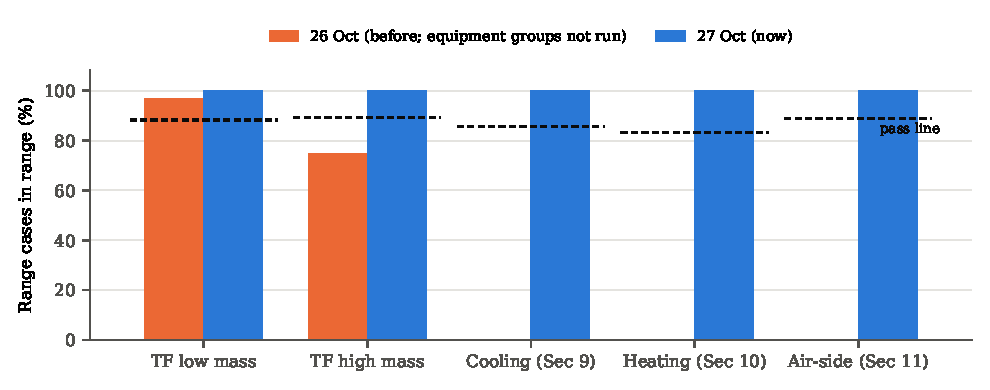
\includegraphics[width=0.95\textwidth]{figures/fig_groups.pdf}
\caption{Annex A3 graded groups, before and after. Dashed line = minimum fraction in range to pass.}\label{fig:groups}\end{figure}

\begin{table}[h]\centering\small
\caption{Annex A3 test-group outcome (official weather files).}\label{tab:groups}
\begin{tabular}{lcccc}\toprule
Group & 26 Oct (GUI) & 27 Oct & Needed & Verdict\\\midrule
Thermal fabric, low mass (A3-1, A3-3) & 33/34 & 34/34 & 30 & pass\\
Thermal fabric, high mass (A3-4, A3-6) & 21/28 & 28/28 & 25 & pass\\
Cooling equipment (A3-7) & not run & 14/14 & 12 & pass\\
Heating equipment (A3-8) & not run & 6/6 & 5 & pass\\
Air-side HVAC (A3-9) & not run & 54/54 & 48 & pass\\\midrule
All range cases & 54/136 & 136/136 & & 5/5 groups\\\bottomrule
\end{tabular}\end{table}

\paragraph{Section 7.} All 52 cases ran with 0 severe errors: 600--695, 900--995, 960, the six free-float cases, and
the in-depth cases 195--470, 800 and 810. Base cases: 600 heating 4.301 / cooling 6.015\,MWh; 900 heating 1.661 /
cooling 2.506\,MWh. Every case lies inside the spread of the example programs, except two on the edge
(695 cooling 9.175 vs maximum 9.172; 290 cooling equal to the maximum). With Pinocchio-EP's normal defaults (no
profile), 900 cooling is 2.936\,MWh, out of range. This is expected: a normal project keeps its real terrain and
daylight saving time.

\paragraph{Section 9.} All 34 cases ran.
\begin{itemize}
\item CE100--CE200 against the quasi-analytical solutions: total energy 0.3--1.8\,\% low, mean COP $-$0.1 to +1.2\,\%,
latent coil load within 0.03\,\%.
\item CE300 annual cooling energy: 35\,039\,kWh (range 33\,497--37\,023).
\end{itemize}
\paragraph{Section 10.}
\begin{itemize}
\item HE100 furnace input 77.756\,GJ against an analytical 77.713\,GJ.
\item HE210 52.694\,GJ (range 49.86--55.11), fan energy 293.9\,kWh.
\item All six ranges pass even at one time step per hour.
\end{itemize}
\paragraph{Section 11.} 54/54 ranged quantities pass. Five VAV cases retain 0.3--1.6\,\% hour-to-hour noise; their
24-hour medians also score 54/54.

\paragraph{Informative sections.}
\begin{itemize}
\item \textbf{Section 6:} the engine reproduces the EPW to $10^{-5}$. 55 of 60 annual incident-solar values are
inside the example range; the other five are at most 0.34\,\% below it.
\item \textbf{Section 8:} 16 of 17 cases ran on the new Kiva support, converged and within $-$7.4 to +1.2\,\% of
the verified numerical models; GC10a cannot be represented in Kiva.
\item \textbf{Section 12:} 38 of 58 results are inside the informative B22 ranges. There is a low bias in the
window-related terms whose cause is not yet found; nothing was tuned.
\end{itemize}

\paragraph{Section 13 (ETNA).}
\begin{itemize}
\item \textbf{``1'' cases:} all within the measurement uncertainty in every best-steady-state hour
(Figure~\ref{fig:etna}).
\item \textbf{Time step:} for a model built from the normative specification it barely matters (under 0.1\,\% from 4
to 60 per hour). The 4--11$\times$ errors in the first study came only from the import cap applied to the
informative input.
\item \textbf{ET100A3/B3:} they need the modeller's interior-convection choice. FisherPedersen is fatal in
EnergyPlus~26.1, so CeilingDiffuser is used. With the measured supply airflow (a normative input column) imposed,
the results are +0.77\,\% and +1.04\,\%, slightly outside $\pm u$ (0.7 / 0.9\,\%). Without it they are $-$8.5 and
$-$8.3\,\%. The airflow was added after the first run, which is disclosed in the results.
\end{itemize}

\begin{figure}[h]\centering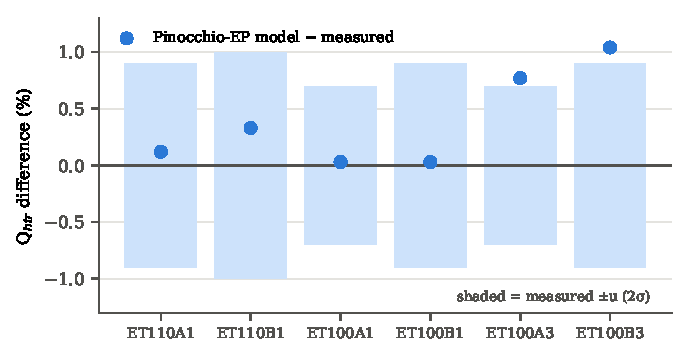
\includegraphics[width=0.6\textwidth]{figures/fig_etna.pdf}
\caption{ETNA: modelled minus measured best-steady-state heater energy. Shaded band = measured $\pm u$.}\label{fig:etna}\end{figure}

\section{Defects found outside Pinocchio-EP}
\begin{description}
\item[EnergyPlus 26.1] \leavevmode
\begin{itemize}
\item The FisherPedersenCeilingDiffuser keys are accepted by the IDD but fatal in \code{MultipleSurface}.
\item \code{LockoutWithCompressor} is ignored on a load-controlled UnitarySystem (CE410 = CE400).
\item \code{EconomizerFirst} staging segfaults.
\item The EPW albedo column is ignored.
\item Wind direction is interpolated straight through north.
\end{itemize}
\item[Standard 140 files] \leavevmode
\begin{itemize}
\item The equation of time in A1.5 uses $(n-81)$; it should be $(n-1)$.
\item The \code{WD400.tmy3} header site differs from the EPW and the text.
\item The local-standard-time column of the TMY files is 30 minutes early.
\item \code{HE100W}--\code{HE140W.WY2} repeat one hour stamp.
\end{itemize}
\end{description}

\section{Status and remaining steps}
All graded tests pass and the required Annex~A2 reports exist. Pinocchio-EP can declare conformance once two
things are done (90.1-2022 \S12.4.1.4):
\begin{enumerate}
\item the exact tested build is released, with its version stamp;
\item the results, input files and modeller reports are posted publicly.
\end{enumerate}
Remaining limits:
\begin{itemize}
\item GC10a and the near-surface ground temperatures (Kiva);
\item the Section~12 P-series and its bias;
\item ETNA's parallel conduction paths need IDF import, because the native face editor cannot split a face.
\end{itemize}

\section*{Reproducibility}
Harnesses: \code{pinocchio-ep/tools/std140/\{tf,et,ce,he,ae,wd,gc,class2\}}. Results, inputs, outputs and filled
workbooks: \code{ashrae140/results/}. Code changes: \code{results/01\_software/code/}.

\begin{thebibliography}{9}\small
\bibitem{s140} ANSI/ASHRAE Standard 140-2023, \emph{Method of Test for Evaluating Building Performance Simulation Software}, with Addendum a (2025) and Addendum b (2026).
\bibitem{acc} ASHRAE, Standard 140-2023 accompanying files, data.ashrae.org/standard140.
\bibitem{s901} ANSI/ASHRAE/IES Standard 90.1-2022, Section 12.4.1.4.
\bibitem{eplus} U.S. DOE, EnergyPlus 26.1.0.
\end{thebibliography}
\end{document}
